\documentclass[aspectratio=169,11pt,t]{beamer}

% ============================================================
% Theme and typography
% ============================================================

\usetheme{Madrid}
\usecolortheme{default}
\usefonttheme{professionalfonts}

\setbeamertemplate{navigation symbols}{}
\setbeamertemplate{headline}{}

\setbeamertemplate{footline}{%
  \leavevmode\hbox{%
  \begin{beamercolorbox}[wd=.82\paperwidth,ht=2.5ex,dp=1.0ex,leftskip=.8em]{author in head/foot}
    CSCI 2406 --- Computer Architecture \& Organization (ARM / RISC Reference)
  \end{beamercolorbox}%
  \begin{beamercolorbox}[wd=.18\paperwidth,ht=2.5ex,dp=1.0ex,rightskip=.8em]{date in head/foot}
    \hfill\insertframenumber/\inserttotalframenumber
  \end{beamercolorbox}}
}

\setbeamersize{
  text margin left=0.65cm,
  text margin right=0.65cm
}

\setbeamerfont{frametitle}{size=\Large, series=\bfseries}
\setbeamerfont{block title}{size=\normalsize, series=\bfseries}
\setbeamertemplate{blocks}[rounded][shadow=false]

% Block vertical padding adjustments
\addtobeamertemplate{block begin}{\vspace{0.1em}}{\vspace{0.1em}}
\addtobeamertemplate{block end}{}{\vspace{0.2em}}

% Base list item separation
\setbeamertemplate{itemize/enumerate body begin}{\setlength{\itemsep}{4pt}}
\setbeamertemplate{itemize/enumerate subbody begin}{\setlength{\itemsep}{2pt}}

% ============================================================
% Packages
% ============================================================

\usepackage[T1]{fontenc}
\usepackage{lmodern}
\usepackage{amsmath}
\usepackage{booktabs}
\usepackage{array}
\usepackage{colortbl}
\usepackage{tikz}

\usetikzlibrary{
  arrows.meta,
  positioning,
  shapes.geometric,
  calc,
  decorations.pathreplacing
}

% ============================================================
% Colors
% ============================================================

\definecolor{navy}{RGB}{24,43,68}
\definecolor{deepblue}{RGB}{45,88,130}
\definecolor{lightblue}{RGB}{235,242,250}
\definecolor{softgray}{RGB}{245,247,250}
\definecolor{darkgray}{RGB}{25,28,32}
\definecolor{gold}{RGB}{200,145,35}

\setbeamercolor{palette primary}{bg=navy,fg=white}
\setbeamercolor{palette secondary}{bg=deepblue,fg=white}
\setbeamercolor{frametitle}{bg=navy,fg=white}
\setbeamercolor{title}{fg=white}
\setbeamercolor{subtitle}{fg=white}
\setbeamercolor{author}{fg=white}
\setbeamercolor{date}{fg=white}
\setbeamercolor{titlelike}{fg=white}
\setbeamercolor{block title}{bg=deepblue,fg=white}
\setbeamercolor{block body}{bg=lightblue,fg=darkgray}
\setbeamercolor{normal text}{fg=darkgray,bg=white}

% ============================================================
% Formatting shortcuts
% ============================================================

\setlength{\parskip}{0pt}

\newcommand{\key}[1]{\textbf{#1}}
\newcommand{\bits}[1]{\texttt{#1}}
\newcommand{\hex}[1]{\texttt{0x#1}}
\newcommand{\code}[1]{\texttt{#1}}

% Section divider macro
\newcommand{\sectiondivider}[2]{%
\begin{frame}[plain]
\begin{tikzpicture}[remember picture,overlay]
\fill[navy] (current page.south west) rectangle (current page.north east);
\fill[gold] (current page.south west) rectangle ([yshift=.15cm]current page.south east);
\end{tikzpicture}
\vspace{1.5cm}
\begin{minipage}{0.85\textwidth}
{\color{gold}\large\bfseries #1\par}
\vspace{0.3cm}
{\color{white}\fontsize{22}{26}\selectfont\bfseries #2\par}
\end{minipage}
\end{frame}
}

% ============================================================
% Metadata
% ============================================================

\title[Topic 2]{
  RISC Principles and ARM Architecture
}

\subtitle{
  RISC vs.\ CISC, ARM Architectural Foundations,\\
  Programmer-Visible State, and Instruction Categories
}

\author{
  Computer Architecture \& Organization
}

\date{Topic 2}

% ============================================================
% Presentation Body (35 Frames Total)
% ============================================================

\begin{document}

% --- Slide 1: Title Slide ---
\begin{frame}[plain]
\begin{tikzpicture}[remember picture,overlay]
\fill[navy] (current page.south west) rectangle (current page.north east);
\fill[gold] (current page.south west) rectangle ([yshift=.18cm]current page.south east);
\end{tikzpicture}
\vspace{1.0cm}
\begin{minipage}{0.9\textwidth}
{\color{gold}\large\bfseries CSCI 2406: Topic 02\par}
\vspace{0.3cm}
{\color{white}\fontsize{20}{24}\selectfont\bfseries RISC Principles and ARM Architecture\par}
\vspace{0.3cm}
{\color{lightblue}\normalsize RISC Design Philosophy, Load/Store Model, AArch32 Programmer-Visible State, and Core Instruction Classes\par}
\vspace{0.6cm}
{\color{softgray}\small Computer Architecture \& Organization \quad\textbar\quad Topic 2\par}
\end{minipage}
\end{frame}

% --- Slide 2: Topic Roadmap ---
\begin{frame}{Topic 2 Technical Roadmap}
    \begin{block}{Topic Objective}
        Analyze the architectural philosophy of Reduced Instruction Set Computers (RISC) and examine how ARM32 / AArch32 realizes this model via registers, control flags, and instruction classes.
    \end{block}
    \vspace{0.4em}
    \begin{itemize}
        \item \key{Section 1}: RISC Design Principles and the Load/Store Paradigm
        \item \key{Section 2}: CISC vs.\ RISC Architectural Trade-Offs
        \item \key{Section 3}: ARM Architectural Overview and Execution States
        \item \key{Section 4}: Registers and Programmer-Visible State (\code{r0}--\code{r15}, \code{cpsr})
        \item \key{Section 5}: Core Instruction Classes: Data Processing, Memory, and Control Flow
        \item \key{Section 6}: Topic Summary and Worked Self-Test Exercises
    \end{itemize}
\end{frame}

% ============================================================
% SECTION 1
% ============================================================
\sectiondivider{Section 01}{RISC Design Principles \&\\the Load/Store Paradigm}

% --- Slide 4: Core RISC Principles ---
\begin{frame}{Foundational RISC Design Principles}
    Reduced Instruction Set Computers (RISC) optimize the hardware-software interface by prioritizing simplicity and regularity:
    \vspace{0.2em}
    \begin{itemize}
        \item \key{Simpler Control Circuitry}: Regular instruction formats and orthogonal opcodes drastically reduce decode and control unit complexity.
        \item \key{Smaller Silicon Footprint}: Eliminating complex microcoded multi-cycle instructions frees die area for larger register files and caches.
        \item \key{Lower Energy Consumption}: Streamlined decoding reduces gate switching activity, yielding high performance-per-watt.
        \item \key{Predictable Pipelining}: Uniform instruction lengths ensure smooth, hazard-free pipeline flow.
    \end{itemize}
\end{frame}

% --- Slide 5: The Load/Store Model ---
\begin{frame}{The Load/Store Architectural Paradigm}
    \begin{block}{Separation of Memory Access and Computation}
        In a pure RISC architecture, data processing instructions (arithmetic, logic) operate \key{exclusively on registers}. Memory is accessed strictly through dedicated \key{load} and \key{store} instructions.
    \end{block}
    \vspace{0.3em}
    \begin{columns}[T]
        \begin{column}{0.48\textwidth}
            \begin{block}{Arithmetic Isolation}
                \begin{itemize}
                    \item ALU inputs must reside in the register file.
                    \item ALU outputs are committed to a register.
                    \item No arithmetic instruction can target a memory address directly.
                \end{itemize}
            \end{block}
        \end{column}
        \begin{column}{0.48\textwidth}
            \begin{block}{Explicit Memory Staging}
                \begin{itemize}
                    \item \code{ldr}: Reads data from memory into a register.
                    \item \code{str}: Writes data from a register into memory.
                    \item Simplifies pipeline address generation and memory stages.
                \end{itemize}
            \end{block}
        \end{column}
    \end{columns}
\end{frame}

% --- Slide 6: The Load/Store Execution Sequence ---
\begin{frame}{Executing Memory Mutation in RISC}
    To mutate a variable stored in RAM (e.g., \code{x = x + 5}), a RISC processor strictly sequences three distinct operations:
    \vspace{0.3em}
    \begin{enumerate}
        \item \key{Load Stage}: Read the variable from memory address \code{[r0]} into working register \code{r1}.
        \item \key{Compute Stage}: Perform register-to-register addition using immediate value \code{\#5}.
        \item \key{Store Stage}: Write modified value in \code{r1} back to memory address \code{[r0]}.
    \end{enumerate}
    \vspace{0.2em}
    \begin{center}
        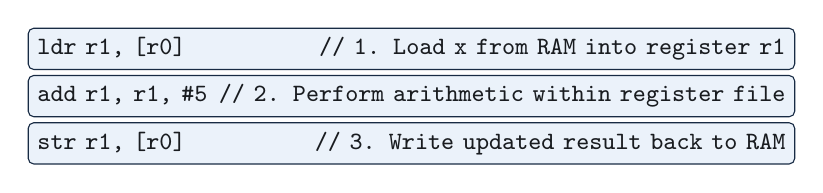
\begin{tikzpicture}[node distance=0.6cm, auto,
            codebox/.style={rectangle, draw=navy, fill=lightblue, text=darkgray, font=\small\ttfamily, text width=9.5cm, align=left, rounded corners=2pt, minimum height=0.45cm}]
            \node [codebox] (c1) {ldr r1, [r0] \hfill // 1. Load x from RAM into register r1};
            \node [codebox, below of=c1] (c2) {add r1, r1, \#5 \hfill // 2. Perform arithmetic within register file};
            \node [codebox, below of=c2] (c3) {str r1, [r0] \hfill // 3. Write updated result back to RAM};
        \end{tikzpicture}
    \end{center}
\end{frame}

% --- Slide 7: Datapath Isolation Diagram ---
\begin{frame}{Visualizing the Load/Store Isolation}
    \begin{center}
        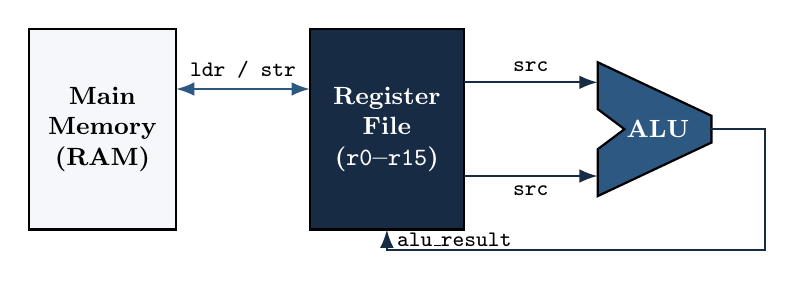
\begin{tikzpicture}[scale=0.85, every node/.style={font=\footnotesize}]
            % RAM Box
            \draw[thick, fill=softgray, text=navy] (0,0.5) rectangle (2.2,3.5);
            \node[font=\small\bfseries, align=center] at (1.1,2.0) {Main\\Memory\\(RAM)};
            
            % Register File Box
            \draw[thick, fill=navy, text=white] (4.2,0.5) rectangle (6.5,3.5);
            \node[font=\small\bfseries, align=center, text=white] at (5.35,2.0) {Register\\File\\(\code{r0}--\code{r15})};
            
            % ALU Box
            \draw[thick, fill=deepblue, text=white] (8.5,1.0) -- (10.2,1.8) -- (10.2,2.2) -- (8.5,3.0) -- (8.5,2.3) -- (8.9,2.0) -- (8.5,1.7) -- cycle;
            \node[font=\small\bfseries, text=white] at (9.4,2.0) {ALU};
            
            % Arrows
            \draw[thick, Latex-Latex, draw=deepblue] (2.2,2.6) -- node[above]{\code{ldr / str}} (4.2,2.6);
            \draw[thick, -Latex, draw=navy] (6.5,2.7) -- node[above]{\code{src}} (8.5,2.7);
            \draw[thick, -Latex, draw=navy] (6.5,1.3) -- node[below]{\code{src}} (8.5,1.3);
            \draw[thick, -Latex, draw=navy] (10.2,2.0) -- (11.0,2.0) -- (11.0,0.2) -- (5.35,0.2) -- node[right]{\code{alu\_result}} (5.35,0.5);
        \end{tikzpicture}
    \end{center}
    \begin{itemize}
        \item The ALU is completely decoupled from the memory bus.
        \item Memory interactions occur exclusively across the register file boundary.
    \end{itemize}
\end{frame}

% ============================================================
% SECTION 2
% ============================================================
\sectiondivider{Section 02}{CISC versus RISC\\Architectural Trade-Offs}

% --- Slide 9: CISC Philosophy ---
\begin{frame}{Complex Instruction Set Computers (CISC)}
    CISC architectures maximize work accomplished per individual instruction:
    \vspace{0.2em}
    \begin{itemize}
        \item \key{Rich, Multi-Step Operations}: A single instruction combines memory fetching, arithmetic calculation, and memory write-back.
        \item \key{Direct Memory Arithmetic}: Instructions can operate directly on operands residing in memory (e.g., \code{add [eax], ebx}).
        \item \key{Variable-Length Formats}: Instruction encodings range from 1 to 15 bytes, requiring complex multi-stage decoders.
        \item \key{Dense Static Code}: High semantic density minimizes program size in RAM.
    \end{itemize}
    \vspace{0.2em}
    \begin{alertblock}{Design Penalty}
        Heavy silicon area and energy cost allocated to instruction decoding and complex hardware microcode control paths.
    \end{alertblock}
\end{frame}

% --- Slide 10: Concrete Comparison: x += 5 ---
\begin{frame}{Code Comparison: Implementing \code{x += 5}}
    Consider incrementing memory variable \code{x} by immediate constant 5:
    \vspace{0.3em}
    \begin{columns}[T]
        \begin{column}{0.48\textwidth}
            \begin{block}{CISC Implementation (x86)}
                \begin{itemize}
                    \item \textbf{Instruction}:
                    \code{add DWORD PTR [x], 5}
                    \item Single variable-length instruction.
                    \item CPU decodes operand, issues memory read, performs ALU add, and writes to memory in microcode.
                    \item Compact binary size, but complex execution timing.
                \end{itemize}
            \end{block}
        \end{column}
        \begin{column}{0.48\textwidth}
            \begin{block}{RISC Implementation (ARM32)}
                \begin{itemize}
                    \item \textbf{Instruction Stream}:
                    \begin{itemize}
                        \item \code{ldr r1, [x]}
                        \item \code{add r1, r1, \#5}
                        \item \code{str r1, [x]}
                    \end{itemize}
                    \item Three fixed 32-bit instructions.
                    \item Higher instruction count, but simple 1-cycle decode and pipeline predictability.
                \end{itemize}
            \end{block}
        \end{column}
    \end{columns}
\end{frame}

% --- Slide 11: Trade-Off Matrix ---
\begin{frame}{CISC vs. RISC Trade-Off Matrix}
    \begin{table}[]
        \centering
        \small
        \begin{tabular}{p{3.0cm} p{4.5cm} p{4.5cm}}
            \toprule
            \textbf{Dimension} & \textbf{CISC (e.g., x86-64)} & \textbf{RISC (e.g., ARM, RISC-V)} \\
            \midrule
            \key{Instruction Size} & Variable (1 to 15 bytes) & Fixed (typically 32-bit) \\
            \key{Memory Access} & Combined with computation & Strict Load/Store only \\
            \key{Addressing Modes} & Many, complex modes & Few, regular modes \\
            \key{Decode Complexity} & High (requires decode ROM/$\mu$ops) & Low (hardwired, orthogonal fields) \\
            \key{Register Count} & Fewer visible registers ($8$--$16$) & Larger register files ($16$--$32+$) \\
            \key{Pipelining} & Difficult due to multi-cycle instructions & Highly efficient and deterministic \\
            \bottomrule
        \end{tabular}
    \end{table}
\end{frame}

% ============================================================
% SECTION 3
% ============================================================
\sectiondivider{Section 03}{ARM Architectural Overview\\and Execution States}

% --- Slide 13: ARM Architecture Overview ---
\begin{frame}{ARM Architecture Overview}
    \key{ARM} is a world-standard RISC instruction set architecture family based on regularity, register-centric computation, and explicit memory access:
    \vspace{0.2em}
    \begin{itemize}
        \item Developed by Arm Ltd.; licensed to semiconductor designers worldwide (Apple, Qualcomm, AWS, NXP).
        \item \key{Target Paradigm}: High computational throughput per milliwatt, ideal for battery-constrained mobile devices and dense cloud datacenters.
        \item \key{Course Baseline}: We utilize \key{ARM32 / AArch32} as our primary model for assembly analysis, register behavior, and microarchitectural design.
    \end{itemize}
    \vspace{0.2em}
    \begin{block}{Architectural Contract vs.\ Microarchitecture}
        The ARM ISA guarantees bit-exact software execution across cores ranging from simple in-order microcontrollers to 8-wide superscalar engines.
    \end{block}
\end{frame}

% --- Slide 14: Fixed-Width Instruction Encoding ---
\begin{frame}{ARM Fixed-Width 32-Bit Instruction Encoding}
    In standard ARM state, every instruction is encoded into an exact \key{32-bit word}:
    \vspace{0.4em}
    \begin{center}
        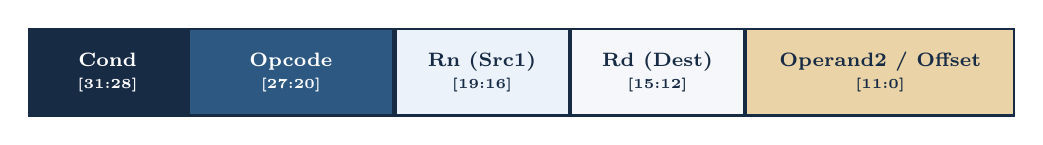
\begin{tikzpicture}[
            scale=1.0,
            fld/.style={draw=navy, thick, minimum height=1.1cm, align=center, font=\scriptsize\bfseries}
        ]
            % Cond [31:28] (4 bits)
            \node[fld, fill=navy, text=white, minimum width=2.0cm] (cond) at (0,0) {
                Cond\\{\tiny[31:28]}
            };
            % Opcode [27:20] (8 bits)
            \node[fld, fill=deepblue, text=white, minimum width=2.6cm, right=0cm of cond] (op) {
                Opcode\\{\tiny[27:20]}
            };
            % Rn / Src1 [19:16] (4 bits)
            \node[fld, fill=lightblue, text=navy, minimum width=2.2cm, right=0cm of op] (rn) {
                Rn (Src1)\\{\tiny[19:16]}
            };
            % Rd / Dest [15:12] (4 bits)
            \node[fld, fill=softgray, text=navy, minimum width=2.2cm, right=0cm of rn] (rd) {
                Rd (Dest)\\{\tiny[15:12]}
            };
            % Operand2 / Offset [11:0] (12 bits)
            \node[fld, fill=gold!40, text=navy, minimum width=3.4cm, right=0cm of rd] (op2) {
                Operand2 / Offset\\{\tiny[11:0]}
            };
        \end{tikzpicture}
    \end{center}
    \vspace{0.2em}
    \begin{itemize}
        \item \key{Simplified Alignment}: Instructions always align on 4-byte boundaries, eliminating unaligned instruction fetch penalties.
        \item \key{Consistent Field Placement}: Source register (\code{rn}) and destination register (\code{rd}) specifiers occupy identical bit locations across instruction families.
        \item \key{Datapath Reuse}: Common field placement minimizes multiplexer routing in the decode stage.
    \end{itemize}
\end{frame}

% --- Slide 15: ARM Execution States ---
\begin{frame}{AArch32 Execution States: ARM vs. Thumb}
    The AArch32 architecture supports two primary operational instruction states:
    \vspace{0.3em}
    \begin{columns}[T]
        \begin{column}{0.48\textwidth}
            \begin{block}{ARM State}
                \begin{itemize}
                    \item Fixed-width 32-bit encodings.
                    \item Full architectural feature access: hardware conditional execution on all instructions.
                    \item Maximizes processing performance and ALU flexibility.
                \end{itemize}
            \end{block}
        \end{column}
        \begin{column}{0.48\textwidth}
            \begin{block}{Thumb / Thumb-2 State}
                \begin{itemize}
                    \item Variable mixture of 16-bit and 32-bit encodings.
                    \item Compresses code size by up to 35\% for memory-constrained embedded ROM/Flash.
                    \item Operates on the exact same register set.
                \end{itemize}
            \end{block}
        \end{column}
    \end{columns}
    \vspace{0.2em}
    \begin{block}{Architectural Commonality}
        Both states share the underlying 32-bit register model (\code{r0}--\code{r15}) and status flags (\code{cpsr}).
    \end{block}
\end{frame}

% ============================================================
% SECTION 4
% ============================================================
\sectiondivider{Section 04}{Registers and Programmer-Visible State}

% --- Slide 17: ARM32 Register Model ---
\begin{frame}{ARM32 Programmer-Visible Register File}
    AArch32 exposes \key{16 visible 32-bit general-purpose registers} (\code{r0}--\code{r15}) plus the \code{cpsr}:
    \vspace{0.2em}
    \begin{center}
        \small
        \begin{tabular}{p{2.5cm} p{3.2cm} p{5.5cm}}
            \toprule
            \textbf{Register} & \textbf{Architectural Role} & \textbf{Standard Software Convention} \\
            \midrule
            \code{r0}--\code{r3} & General Purpose & Function argument inputs / return values \\
            \code{r4}--\code{r11} & General Purpose & Callee-saved local variables \\
            \code{r12} (\code{ip}) & General Purpose & Intra-procedure call scratch register \\
            \rowcolor{gold!15} \code{r13} (\code{sp}) & \key{Stack Pointer} & Holds memory address of the current stack frame \\
            \rowcolor{gold!15} \code{r14} (\code{lr}) & \key{Link Register} & Holds return address for function calls (\code{bl}) \\
            \rowcolor{gold!15} \code{r15} (\code{pc}) & \key{Program Counter} & Holds the memory address of the executing instruction \\
            \bottomrule
        \end{tabular}
    \end{center}
\end{frame}

% --- Slide 18: The Program Counter (PC) Deep Dive ---
\begin{frame}{The Program Counter (\code{r15} / \code{pc})}
    The \key{Program Counter} tracks the execution stream in memory:
    \vspace{0.2em}
    \begin{itemize}
        \item In \key{AArch32}, \code{pc} is architecturally mapped directly to \key{\code{r15}}.
        \item Software can read \code{r15} or write to it directly using standard data instructions (e.g., \code{mov pc, lr} to return from a function).
        \item \key{Pipelining Offset}: Reading \code{pc} in ARM state returns $\text{current instruction address} + 8$ due to the 3-stage fetch-decode-execute pipeline prefetching.
    \end{itemize}
    \vspace{0.2em}
    \begin{alertblock}{Important Evolution: AArch64 Architectural Difference}
        In 64-bit ARM (\key{AArch64}), \code{pc} is \textbf{not} a general-purpose register. It cannot be targeted by arithmetic instructions and can only be updated through dedicated branch/jump operations.
    \end{alertblock}
\end{frame}

% --- Slide 19: CPSR and Condition Flags ---
\begin{frame}{Current Program Status Register (CPSR)}
    The \key{CPSR} holds runtime system status, processor mode bits, and arithmetic condition flags:
    \vspace{0.2em}
    \begin{center}
        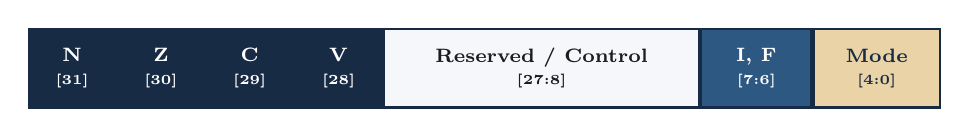
\begin{tikzpicture}[
            scale=1.0,
            fld/.style={draw=navy, thick, minimum height=1.0cm, align=center, font=\scriptsize\bfseries}
        ]
            % CPSR bit field diagram
            \node[fld, fill=navy, text=white, minimum width=1.1cm] (n) at (0,0) {N\\{\tiny[31]}};
            \node[fld, fill=navy, text=white, minimum width=1.1cm, right=0cm of n] (z) {Z\\{\tiny[30]}};
            \node[fld, fill=navy, text=white, minimum width=1.1cm, right=0cm of z] (c) {C\\{\tiny[29]}};
            \node[fld, fill=navy, text=white, minimum width=1.1cm, right=0cm of c] (v) {V\\{\tiny[28]}};
            \node[fld, fill=softgray, text=darkgray, minimum width=4.0cm, right=0cm of v] (res) {Reserved / Control\\{\tiny[27:8]}};
            \node[fld, fill=deepblue, text=white, minimum width=1.4cm, right=0cm of res] (ifg) {I, F\\{\tiny[7:6]}};
            \node[fld, fill=gold!40, text=navy, minimum width=1.6cm, right=0cm of ifg] (mode) {Mode\\{\tiny[4:0]}};
        \end{tikzpicture}
    \end{center}
    \vspace{0.1em}
    \begin{block}{The Arithmetic Condition Flags (NZCV)}
        \begin{itemize}
            \item \key{N (Negative)}: Set if the result bit 31 is 1 (negative signed value).
            \item \key{Z (Zero)}: Set if the result of the operation equals 0.
            \item \key{C (Carry)}: Set if an unsigned operation generated an arithmetic carry-out or non-borrow.
            \item \key{V (oVerflow)}: Set if a signed operation exceeded 32-bit 2's complement range.
        \end{itemize}
    \end{block}
\end{frame}

% --- Slide 20: Architectural State Summary ---
\begin{frame}{Complete ARM Architectural State}
    \begin{block}{Formal Definition}
        \key{Architectural State} comprises all hardware register contents and memory state that must be preserved to guarantee bit-exact program resumption.
    \end{block}
    \vspace{0.3em}
    \begin{columns}[T]
        \begin{column}{0.48\textwidth}
            \begin{block}{Programmer-Visible Components}
                \begin{itemize}
                    \item 16 General Registers: \code{r0}--\code{r15}.
                    \item Dedicated Roles: \code{sp}, \code{lr}, \code{pc}.
                    \item Status State: \code{cpsr} (NZCV flags).
                    \item Addressable memory space (RAM).
                \end{itemize}
            \end{block}
        \end{column}
        \begin{column}{0.48\textwidth}
            \begin{block}{State Transitions}
                \begin{itemize}
                    \item Instructions execute by transitioning state:
                    $$\text{State}_{t+1} \leftarrow f(\text{State}_t, \text{Instruction})$$
                    \item Microarchitectural structures (caches, pipelines) change physically but remain invisible.
                \end{itemize}
            \end{block}
        \end{column}
    \end{columns}
\end{frame}

% ============================================================
% SECTION 5
% ============================================================
\sectiondivider{Section 05}{Core AArch32 Instruction Classes}

% --- Slide 22: The Three Instruction Classes ---
\begin{frame}{AArch32 Instruction Categories}
    Every operation in the ARM ISA partitions into one of three core functional classes:
    \vspace{0.4em}
    \begin{columns}[T]
        \begin{column}{0.32\textwidth}
            \begin{block}{1. Data Processing}
                \begin{itemize}
                    \item Arithmetic \& logic.
                    \item Register-only inputs.
                    \item Optional flag updates.
                    \item Examples: \code{add}, \code{sub}, \code{mul}, \code{mov}, \code{cmp}.
                \end{itemize}
            \end{block}
        \end{column}
        \begin{column}{0.32\textwidth}
            \begin{block}{2. Memory Access}
                \begin{itemize}
                    \item Transfers between RAM and registers.
                    \item Base register addressing.
                    \item Examples: \code{ldr}, \code{str}, \code{ldrb}, \code{strb}.
                \end{itemize}
            \end{block}
        \end{column}
        \begin{column}{0.32\textwidth}
            \begin{block}{3. Control Flow}
                \begin{itemize}
                    \item Branching and jumps.
                    \item Direct mutation of \code{pc}.
                    \item Conditional execution.
                    \item Examples: \code{b}, \code{beq}, \code{bne}, \code{blt}, \code{bl}.
                \end{itemize}
            \end{block}
        \end{column}
    \end{columns}
\end{frame}

% --- Slide 23: Data Processing Instructions ---
\begin{frame}{Class 1: Data Processing Instructions}
    Data processing instructions compute mathematical or logical operations within registers:
    \vspace{0.3em}
    \begin{center}
        \small
        \begin{tabular}{p{3.2cm} p{3.8cm} p{4.5cm}}
            \toprule
            \textbf{Instruction Syntax} & \textbf{Semantic Operation} & \textbf{Architectural Effect} \\
            \midrule
            \code{add r3, r1, r2} & Addition & $\code{r3} \leftarrow \code{r1} + \code{r2}$ \\
            \code{sub r3, r3, r2} & Subtraction & $\code{r3} \leftarrow \code{r3} - \code{r2}$ \\
            \code{mul r3, r1, r2} & Multiplication & $\code{r3} \leftarrow \code{r1} \times \code{r2}$ \\
            \code{mov r3, r4} & Register Transfer & $\code{r3} \leftarrow \code{r4}$ \\
            \code{and r0, r1, r2} & Bitwise Logical AND & $\code{r0} \leftarrow \code{r1} \text{ AND } \code{r2}$ \\
            \code{orr r0, r1, r2} & Bitwise Logical OR & $\code{r0} \leftarrow \code{r1} \text{ OR } \code{r2}$ \\
            \bottomrule
        \end{tabular}
    \end{center}
    \vspace{0.2em}
    \begin{block}{Immediate Constant Variant}
        Operands can be numerical literals: \code{add r1, r1, \#5} adds constant 5 to register \code{r1}.
    \end{block}
\end{frame}

% --- Slide 24: Memory Instructions ---
\begin{frame}{Class 2: Memory Access Instructions}
    Memory access instructions transfer words or bytes between RAM and the CPU register file:
    \vspace{0.3em}
    \begin{center}
        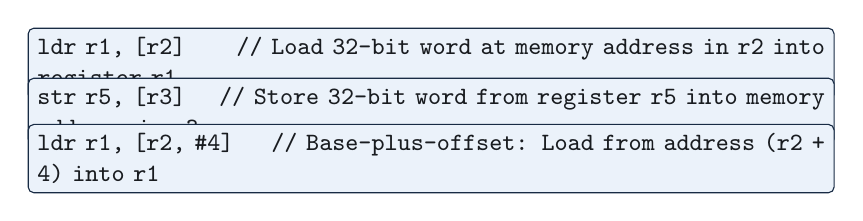
\begin{tikzpicture}[node distance=0.6cm, auto,
            membox/.style={rectangle, draw=navy, fill=lightblue, text=darkgray, font=\small\ttfamily, text width=10.0cm, align=left, rounded corners=2pt, minimum height=0.55cm}]
            \node [membox] (m1) {ldr r1, [r2] \hfill // Load 32-bit word at memory address in r2 into register r1};
            \node [membox, below of=m1] (m2) {str r5, [r3] \hfill // Store 32-bit word from register r5 into memory address in r3};
            \node [membox, below of=m2] (m3) {ldr r1, [r2, \#4] \hfill // Base-plus-offset: Load from address (r2 + 4) into r1};
        \end{tikzpicture}
    \end{center}
    \vspace{0.2em}
    \begin{block}{Bracket Notation \code{[r2]}}
        Brackets represent \key{memory dereferencing}. The register inside brackets contains the memory address pointer; the operation accesses the memory cell at that numerical address.
    \end{block}
\end{frame}

% --- Slide 25: Comparison Instructions ---
\begin{frame}{Comparison Operations and the \code{cmp} Instruction}
    Conditional decision-making begins with explicit comparison instructions:
    \vspace{0.3em}
    \begin{block}{\code{cmp r0, r1} (Compare Operands)}
        \begin{itemize}
            \item Performs internal subtraction: $\text{Temporary} \leftarrow \code{r0} - \code{r1}$.
            \item \key{Discards Result}: The numerical difference is not stored in any register.
            \item \key{Updates CPSR}: Evaluates and sets condition flags (\key{N, Z, C, V}) based on the subtraction.
        \end{itemize}
    \end{block}
    \vspace{0.3em}
    \begin{columns}[T]
        \begin{column}{0.48\textwidth}
            \begin{block}{If $\code{r0} == \code{r1}$}
                $\code{r0} - \code{r1} = 0 \rightarrow$ \key{Z flag set to 1}.
            \end{block}
        \end{column}
        \begin{column}{0.48\textwidth}
            \begin{block}{If $\code{r0} < \code{r1}$}
                $\code{r0} - \code{r1} < 0 \rightarrow$ \key{N flag set to 1}.
            \end{block}
        \end{column}
    \end{columns}
\end{frame}

% --- Slide 26: Class 3: Control Flow Instructions ---
\begin{frame}{Class 3: Control Flow and Branching}
    Branch instructions alter program flow by loading new target addresses into the \code{pc}:
    \vspace{0.3em}
    \begin{columns}[T]
        \begin{column}{0.48\textwidth}
            \begin{block}{Unconditional Branch}
                \code{b target\_label}
                \begin{itemize}
                    \item Forces execution to diverge unconditionally.
                    \item Overwrites \code{pc} with the target address.
                    \item Equivalent to \code{jmp} in x86 assembly.
                \end{itemize}
            \end{block}
        \end{column}
        \begin{column}{0.48\textwidth}
            \begin{block}{Conditional Branches}
                \code{b<cond> target\_label}
                \begin{itemize}
                    \item Evaluates NZCV flags in \code{cpsr}.
                    \item If condition holds true $\rightarrow$ update \code{pc}.
                    \item If false $\rightarrow$ fall through sequentially ($PC \leftarrow PC + 4$).
                \end{itemize}
            \end{block}
        \end{column}
    \end{columns}
    \vspace{0.2em}
    \begin{center}
        \small
        \begin{tabular}{lll}
            \toprule
            \textbf{Mnemonic} & \textbf{Meaning} & \textbf{Tested Flag Condition} \\
            \midrule
            \code{beq} & Branch if Equal & $\text{Z} == 1$ \\
            \code{bne} & Branch if Not Equal & $\text{Z} == 0$ \\
            \code{blt} & Branch if Less Than (Signed) & $\text{N} \neq \text{V}$ \\
            \code{bgt} & Branch if Greater Than (Signed) & $(\text{Z} == 0) \text{ and } (\text{N} == \text{V})$ \\
            \bottomrule
        \end{tabular}
    \end{center}
\end{frame}

% --- Slide 27: Assembly Decisions (Fixed Alignment) ---
\begin{frame}{Assembly Decisions: The Compare-and-Branch Pattern}
    High-level \code{if-else} statements are implemented via a 2-step assembly pattern:
    \vspace{0.3em}
    \begin{columns}[T]
        \begin{column}{0.48\textwidth}
            \begin{block}{Step 1: Evaluate Condition}
                \code{cmp r1, r2}
                \vspace{0.2em}
                \begin{itemize}
                    \item Subtracts \code{r2} from \code{r1} internally.
                    \item Updates \key{NZCV} flags in \code{cpsr}.
                \end{itemize}
            \end{block}
        \end{column}
        \begin{column}{0.48\textwidth}
            \begin{block}{Step 2: Test Flags \& Branch}
                \code{beq equal\_label}
                \vspace{0.2em}
                \begin{itemize}
                    \item Evaluates flag state (e.g., $Z == 1$).
                    \item If true $\rightarrow$ updates \code{pc} to label.
                \end{itemize}
            \end{block}
        \end{column}
    \end{columns}
    \vspace{0.3em}
    \begin{block}{Complete Conditional Pattern}
        \vspace{0.1em}
        \centering
        \small
        \begin{tabular}{@{}ll@{}}
            \code{cmp r1, r2}           & \code{// 1. Compare r1 and r2} \\
            \code{beq equal\_path}       & \code{// 2. If r1 == r2, branch to equal\_path} \\
            \code{sub r0, r1, r2}       & \code{// Fall-through: executed if r1 != r2} \\
            \code{b end\_block}          & \code{// Bypass true-block} \\
            \code{equal\_path:}          & \\
            \code{\quad add r0, r1, r2} & \code{// True-block: executed if r1 == r2} \\
            \code{end\_block:}           & 
        \end{tabular}
        \vspace{0.1em}
    \end{block}
\end{frame}

% --- Slide 28: Labels, Addresses, and PC Mutation ---
\begin{frame}{Labels as Memory Aliases}
    \begin{block}{What is an Assembly Label?}
        An assembly label (e.g., \code{target:}) is a human-readable alias representing the exact numerical \key{memory address} where subsequent instructions reside.
    \end{block}
    \vspace{0.3em}
    \begin{columns}[T]
        \begin{column}{0.5\textwidth}
            \key{Assembly Source Code}:
            \vspace{0.2em}
            \begin{center}
                \begin{minipage}{0.9\textwidth}
                    \code{b compute\_sum \hfill // Branch}\\
                    \code{mov r0, \#0}\\
                    \code{compute\_sum: \hfill // Label}\\
                    \code{add r0, r1, r2 \hfill // Target}
                \end{minipage}
            \end{center}
        \end{column}
        \begin{column}{0.48\textwidth}
            \key{Hardware Memory View}:
            \vspace{0.2em}
            \begin{center}
                \small
                \begin{tabular}{ll}
                    \toprule
                    \textbf{Address} & \textbf{Machine Instruction} \\
                    \midrule
                    \hex{0x00008000} & \code{b +0x8 (\hex{0x00008008})} \\
                    \hex{0x00008004} & \code{mov r0, \#0} \\
                    \rowcolor{gold!20} \hex{0x00008008} & \code{add r0, r1, r2} \\
                    \bottomrule
                \end{tabular}
            \end{center}
        \end{column}
    \end{columns}
    \vspace{0.3em}
    \begin{alertblock}{Execution Safety}
        The branch target must resolve to a valid instruction memory address to prevent invalid opcode crashes.
    \end{alertblock}
\end{frame}

% ============================================================
% SECTION 6
% ============================================================
\sectiondivider{Section 06}{Summary \& Self-Test}

% --- Slide 30: Topic Summary ---
\begin{frame}{Topic 2 Comprehensive Summary}
    \begin{itemize}
        \item \key{RISC Design Philosophy}: Emphasizes simple control circuitry, regular instruction formats, fixed-width encodings, and high energy efficiency.
        \item \key{Load/Store Architecture}: Strict isolation of memory access (\code{ldr}, \code{str}) from computation (\code{add}, \code{sub}).
        \item \key{AArch32 Register File}: 16 visible 32-bit registers (\code{r0}--\code{r15}) where \code{r13} is \code{sp}, \code{r14} is \code{lr}, and \code{r15} is \code{pc}.
        \item \key{Program Counter (\code{pc})}: In AArch32, \code{pc} is accessible as \code{r15} (with $+8$ pipeline offset); in AArch64, \code{pc} is separated from general registers.
        \item \key{Condition Flags (CPSR)}: The \code{cmp} instruction updates \key{N, Z, C, V} flags to drive conditional branches (\code{beq}, \code{bne}, \code{blt}).
        \item \key{Instruction Classes}: All ARM instructions partition into Data Processing, Memory Access, or Control Flow.
    \end{itemize}
\end{frame}

% --- Slide 31: Self-Test: Questions 1 & 2 ---
\begin{frame}{Self-Test: Questions 1 \& 2}
    \begin{block}{Question 1: RISC vs.\ CISC Principles}
        What are the main architectural principles that distinguish RISC from CISC? Why does simpler instruction decoding reduce processor power consumption?
    \end{block}
    \vspace{0.4em}
    \begin{block}{Question 2: The Load/Store Sequence}
        How does the ARM32 instruction sequence below implement an update to a memory variable? Why can't ARM perform this operation in a single arithmetic instruction?
        \begin{center}
            \code{ldr r1, [r0]} \quad $\rightarrow$ \quad \code{add r1, r1, \#5} \quad $\rightarrow$ \quad \code{str r1, [r0]}
        \end{center}
    \end{block}
\end{frame}

% --- Slide 32: Self-Test: Solutions 1 \& 2 ---
\begin{frame}{Self-Test: Solutions 1 \& 2}
    \begin{block}{Solution 1}
        RISC uses fixed-width instructions, a load/store model, and regular operand fields. CISC uses variable-length encodings and direct memory arithmetic. Simpler decoding reduces silicon gate count and dynamic switching activity ($P \propto C \cdot V^2 \cdot f$), lowering power draw.
    \end{block}
    \vspace{0.3em}
    \begin{block}{Solution 2}
        The sequence explicitly stages memory mutation: \code{ldr} loads data into \code{r1}, \code{add} computes in the ALU, and \code{str} writes back to RAM. ARM cannot combine these because the ALU datapath is isolated from memory buses, adhering to the pure RISC load/store principle.
    \end{block}
\end{frame}

% --- Slide 33: Self-Test: Questions 3 & 4 ---
\begin{frame}{Self-Test: Questions 3 \& 4}
    \begin{block}{Question 3: ARM32 Registers and Special Roles}
        Which ARM32 registers are general-purpose operands, and what special architectural roles are assigned to \code{r13}, \code{r14}, and \code{r15}? How is \code{pc} exposed differently in AArch64?
    \end{block}
    \vspace{0.4em}
    \begin{block}{Question 4: Instruction Classes}
        What are the three core instruction classes in AArch32? Give one specific instruction example for each class.
    \end{block}
\end{frame}

% --- Slide 34: Self-Test: Solutions 3 \& 4 ---
\begin{frame}{Self-Test: Solutions 3 \& 4}
    \begin{block}{Solution 3}
        \begin{itemize}
            \item \code{r0}--\code{r12}: General-purpose registers for operands and variables.
            \item \code{r13} (\code{sp}): Stack Pointer; \code{r14} (\code{lr}): Link Register; \code{r15} (\code{pc}): Program Counter.
            \item In AArch64, the \code{pc} is \textbf{not} a general-purpose register and cannot be accessed as a numbered register operand.
        \end{itemize}
    \end{block}
    \vspace{0.3em}
    \begin{block}{Solution 4}
        \begin{enumerate}
            \item \key{Data Processing}: \code{add r3, r1, r2} (computes within registers).
            \item \key{Memory Access}: \code{ldr r1, [r2]} (loads word from memory into register).
            \item \key{Control Flow}: \code{beq target} (conditionally branches by updating \code{pc}).
        \end{enumerate}
    \end{block}
\end{frame}

% --- Slide 35: Self-Test: Question 5 & Solution ---
\begin{frame}{Self-Test: Question 5 \& Solution}
    \begin{block}{Question 5: Compare-and-Branch Execution}
        How do \code{cmp} and a conditional branch such as \code{blt} work together to implement high-level decision making? What register stores the intermediate outcome?
    \end{block}
    \vspace{0.3em}
    \pause
    \begin{block}{Solution 5}
        \begin{itemize}
            \item \code{cmp r0, r1} performs an internal subtraction ($\code{r0} - \code{r1}$), discards the numeric result, and updates the \key{N, Z, C, V} flags in the \key{CPSR} (Current Program Status Register).
            \item \code{blt label} subsequently inspects the flags ($N \neq V$) in the \code{cpsr}. If true, it loads the label address into \code{pc}; otherwise, it falls through to the next instruction.
            \item Intermediate comparison outcome is stored in the \key{CPSR}.
        \end{itemize}
    \end{block}
\end{frame}

\end{document}